\documentclass[12pt,letterpaper]{article}
\usepackage{graphicx}
\DeclareGraphicsExtensions{.pdf,.png,.jpg,.mps}
\usepackage{hyperref} 
\usepackage{amsmath}
\usepackage{amssymb}
\usepackage{natbib}
\usepackage{rotating}
\usepackage{multirow}
\usepackage{hhline}
\usepackage{longtable}
\usepackage[margin=0.75in]{geometry}

 
  
\begin{document}
 
\title{The Future Americans Model: Technical Documentation}
\author{
Dana P. Goldman, University of Southern California\\
\and Duncan Ermini Leaf, University of Southern California
\and Bryan Tysinger, University of Southern California\\
}

\maketitle
\newpage
\tableofcontents
\newpage
\listoffigures
\listoftables
 
\section{Functioning of the dynamic model}
\subsection{Background}
The Future Elderly Model (FEM) is a microsimulation model originally developed out of an effort to 
examine health and health care costs among the elderly Medicare population (age 65+). A description 
of the previous incarnation of the model can be found in \citet{goldman2004health}. The original work was 
founded by the Centers for Medicare and Medicaid Services and carried out by a team of researchers 
composed of Dana P. Goldman, Paul G. Shekelle, Jayanta Bhattacharya, Michael Hurd, Geoffrey F. Joyce, 
Darius N. Lakdawalla, Dawn H. Matsui, Sydne J. Newberry, Constantijn W. A. Panis and Baoping Shang.

Since then various extensions have been implemented to the original model. The most recent version 
now projects health outcomes for all Americans aged 51 and older and uses the Health and Retirement 
Study (HRS) as a host dataset rather than the Medicare Current Beneficiary Survey (MCBS).  The work 
has also been extended to include economic outcomes such as earnings, labor force participation and 
pensions. This work was funded by the National Institute on Aging through its support of the RAND 
Roybal Center for Health Policy Simulation (P30AG024968), the Department of Labor through contract 
J-9-P-2-0033, the National Institutes of Aging through the R01 grant ``Integrated Retirement 
Modeling'' (R01AG030824) and the MacArthur Foundation Research Network on an Aging Society. Finally, 
the computer code of the model was transferred from Stata to C++. This report incorporates these new 
development efforts in the description of the model.
% \todo add description of work extending to ages 25+ (FAM) here

\subsection{Overview}

The defining characteristic of the model is the modeling of real rather than synthetic cohorts, all of whom are followed at the individual level. This allows for more heterogeneity in behavior than would be allowed by a cell-based approach. Also, since the HRS interviews both respondent and spouse, we can link records to calculate household-level outcomes such as net income and Social Security retirement benefits, which depend on the outcomes of both spouses. The omission of the population younger than age 51 sacrifices little generality, since the bulk of expenditure on the public programs we consider occurs after age 50. However, we may fail to capture behavioral responses among the young. 

The model has three core components: 
\begin{itemize}
\item The initial cohort module predicts the economic and health outcomes of new cohorts of 51/52 
year-olds. This module takes in data from the Health and Retirement Study (HRS) and trends calculated 
from other sources. It allows us to ``generate'' cohorts as the simulation proceeds, so that we can 
measure outcomes for the age 51+ population in any given year. 
\item The transition module calculates the probabilities of transiting across various health states 
and financial outcomes. The module takes as inputs risk factors such as smoking, weight, age and 
education, along with lagged health and financial states. This allows for a great deal of 
heterogeneity and fairly general feedback effects. The transition probabilities are estimated from 
the longitudinal data in the Health and Retirement Study (HRS). 
\item The policy outcomes module aggregates projections of individual-level outcomes into policy 
outcomes such as taxes, medical care costs, pension benefits paid, and disability benefits. This 
component takes account of public and private program rules to the extent allowed by the available 
outcomes. Because we have access to HRS-linked restricted data from Social Security records and 
employer pension plans, we are able to realistically model retirement benefit receipt. 
\end{itemize}

\begin{figure}[h]
\centering
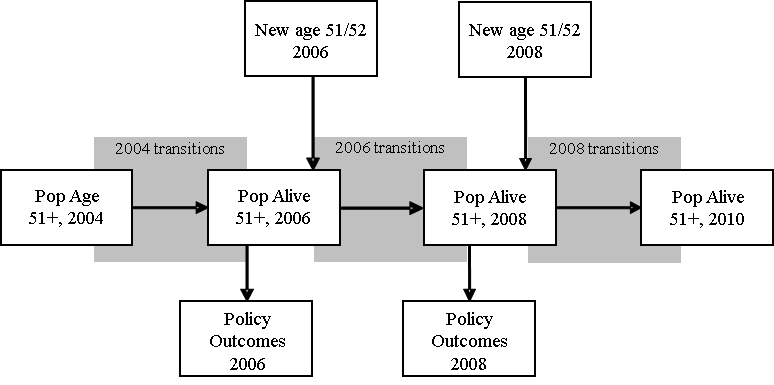
\includegraphics[scale=0.8]{./img/fem_architecture.png}
\caption{Architecture of the FEM}
\label{fig:fem_architecture} 
\end{figure}

Figure \ref{fig:fem_architecture} provides a schematic overview of the model. We start in 2004 with 
an initial population aged 51+ taken from the HRS. We then predict outcomes using our estimated 
transition probabilities (see section \ref{sec:estimation_transition_model}). Those who survive make it to the end of that year, at 
which point we calculate policy outcomes for the year. We then move to the following time period 
(two years later), when a new cohort of 51 and 52 year-olds enters (see section \ref{sec:new_cohorts_model_empirical_strategy}). This entrance 
forms the new age 51+ population, which then proceeds through the transition model as before. This 
process is repeated until we reach the final year of the simulation. 

\subsection{Comparison with other prominent microsimulation models of health expenditures}
The FEM is unique among existing models that make health expenditure projections. It is the only model 
that projects health trends rather than health expenditures. It is also the only model that generates 
mortality out of assumptions on health trends rather than historical time series.

\subsubsection{CBOLT Model}
The Congressional Budget Office (CBO) uses time-series techniques to project health expenditure 
growth in the short term and then makes an assumption on long-term growth. They use a long term 
growth of excess costs of 2.3 percentage points starting in 2020 for Medicare. They then assume a 
reduction in excess cost growth in Medicare of 1.5\% through 2083, leaving a rate of 0.9\% in 2083. 
For non-Medicare spending they assume an annual decline of 4.5\%, leading to an excess growth rate in 
2083 of 0.1\%. 

\subsubsection{Centers for Medicare and Medicaid Services}
The Centers for Medicare and Medicaid Services (CMS) performs an extrapolation of medical expenditures 
over the first ten years, then computes a general equilibrium model for years 25 through 75 and 
linearly interpolates to identify medical expenditures in years 11 through 24 of their estimation. 
The core assumption they use is that excess growth of health expenditures will be one percentage point 
higher per year for years 25-75 (that is if nominal GDP growth is 4\%, health care expenditure growth 
will be 5\%).



\section{Data sources used for estimation}
The Panel Survey of Income Dynamics is the main data source for the model. We estimate models
for assigning characteristics for the replacement cohorts in Replenishing Conditions Module.  These
are summarized in Table \ref{tab:initial_conditions_model}.  We estimate transition models for 
the entire PSID population in the Transition Model Module.  Transitioned outcomes are described in
Table \ref{tab:transition_model}.


\subsection{Panel Survey of Income Dynamics}
The Panel Survey of Income Dynamics (PSID), waves 1999-2013 are used to estimate the transition models. 
PSID interviews occur every two years.  We create a dataset of respondents who have formed their own households, either
as single heads of households, cohabitating partners, or married partners.  These heads, wives, and "wives" (males
are automatically assigned head of household status by the PSID if they are in a couple) respond to the richest
set of PSID questions, including the health questions that are critical for our purposes.

We use all respondents age 25 and older.  When appropriately weighted, the PSID is representative of U.S. households.  
We also use the PSID as the host data for full population simulations that begin in 2009.  Respondents age 25 and 26 
are used as the basis for the synthetic cohorts that we generate, used for replenishing the sample in population 
simulations or as the basis of cohort scenarios.  

The PSID continually adds new cohorts that are descendents (or new partners/spouses of descendents).  Consequently,
updating the simulation to include more recent data is straightforward.
\subsection{Health and Retirement Study}
The Health and Retirement Study (HRS) waves 2000-2008 are used to estimate the transition model. 
Interviews occur every two years. We use the dataset created by RAND (RAND HRS, version K) as our 
basis for the analysis. We use all cohorts in the analysis and consider sampling weights whenever 
appropriate. When appropriately weighted, the HRS in 2004 is representative of U.S. households where 
at least one member is at least 51. The HRS is also used as the host data for the simulation (pop 51+ in 2004) and for new cohorts (aged 51 and 52 in 2004).

The HRS adds new cohorts every six years. Until recently, the latest available cohort had been added 
in 2004, which is why that is the FEM's base year. The FEM is currently being updated to use the 
newly released 2010 data.

%\subsection{Social Security covered earnings files}
To get information on Social Security entitlements of respondents, we match the HRS data to the 
Social Security Covered Earnings files of 1992, 1993, 1998, 2004 and 2006 which provides information on 
earning histories of respondents as well as their entitlement to future Social Security benefits. We 
then construct the average indexed monthly earnings (AIME), the basis for the determination of benefit 
levels, from these earning histories. The AIME is constructed by first indexing using the National 
Wage Index (NWI) to the wage level when the respondent turns age 60. If this occurs after 2008, we 
project the evolution of the NWI using the average annual rate of change of the last 20 years (2.9\% 
nominal). We then take the 35 highest years (if less than 35 years are available, remaining years are 
considered zero earning years) and take the average. We then convert back this annual amount on a 
monthly basis and convert back to \$2004 U.S. dollars using the CPI. Quarters of coverage, which 
determine eligibility to Social Security, are defined as the sum of posted quarters to the file. A 
worker is eligible for Social Security if he has accumulated at least 40 quarters of coverage. A 
worker roughly accumulates a quarter of coverage for every \$4000 of coverage earnings up to a maximum 
of 4 per year. Not all respondents agree to have their record matched. Hence, there is the potential 
for non-representativeness. However, recent studies show that the extent of non-representativeness is 
quite small and that appropriate weighting using HRS weights mostly corrects for this problem 
\citep{kapteyn2006effects}.
%\subsection{National Health Interview Survey}
The National Health Interview Survey (NHIS) contains individual-level data on height, weight, smoking 
status, self-reported chronic conditions, income, education, and demographic variables. It is a 
repeated cross-section done every year for several decades. But the survey design has been 
significantly modified several times. Before year 1997, different subgroups of individuals were asked 
about different sets of chronic conditions, after year 1997, a selected sub-sample of the adults were 
asked a complete set of chronic conditions. The survey questions are quite similar to that in HRS. As 
a result, for projecting the trends of chronic conditions for future 51/52 year-olds, we only use data 
from 1997 to 2010. A review of survey questions is provided in Table \ref{tab:svy_disease_questions}. Information on 
weight and height were asked every year, while information on smoking was asked in selected years before 
year 1997, and has been asked annually since year 1997. 

FEM uses NHIS to project prevalence of chronic conditions in future cohorts of 51-52 year olds.  The
method is discussed in Sections \ref{sec:data_sources_trends_and_baseline_entering_cohorts} and \ref{sec:new_cohorts_model_empirical_strategy}.  FEM
also relies on the Medical Expenditure Panel Survey, a subsample of NHIS respondents, for model estimation.
See section \ref{sec:data_sources_estimation_meps} for a description.


\subsection{Medical Expenditure Panel Survey}
\label{sec:data_sources_estimation_meps}
The Medical Expenditure Panel Survey (MEPS), beginning in 1996, is a set of large-scale surveys of 
families and individuals, their medical providers (doctors, hospitals, pharmacies, etc.), and 
employers across the United States. The Household Component (HC) of the MEPS provides data from 
individual households and their members, which is supplemented by data from their medical providers. 
The Household Component collects data from a representative sub sample of households drawn from the 
previous year's National Health Interview Survey (NHIS). Since NHIS does not include the 
institutionalized population, neither does MEPS: this implies that we can only use the MEPS to 
estimate medical costs for the non-elderly population. Information collected during household 
interviews include: demographic characteristics, health conditions, health status, use of medical 
services, sources of medical payments, and body weight and height. Each year the household survey 
includes approximately 12,000 households or 34,000 individuals. Sample size for those aged 51-64 is 
about 4,500.  MEPS has comparable measures of social-economic (SES) variables as those in HRS, 
including age, race/ethnicity, educational level, census region, and marital status. 

FEM uses MEPS years 2000-2010 for cost estimation.  See Section 
\ref{sec:govt_revenue_and_expenditures_medcost_estimation} for a description.  FEM also
uses MEPS 2001 data for QALY model estimation. This is described in Section 
\ref{sec:estimation_qalys}.


\subsection{Medicare Current Beneficiary Survey}
The Medicare Current Beneficiary Survey (MCBS) is a nationally representative sample of aged, disabled 
and institutionalized Medicare beneficiaries.  The MCBS attempts to interview each respondent twelve 
times over three years, regardless of whether he or she resides in the community, a facility, or 
transitions between community and facility settings. The disabled (under 65 years of age) and 
oldest-old (85 years of age or older) are over-sampled. The first round of interviewing was conducted 
in 1991. Originally, the survey was a longitudinal sample with periodic supplements and indefinite 
periods of participation. In 1994, the MCBS switched to a rotating panel design with limited periods 
of participation. Each fall a new panel is introduced, with a target sample size of 12,000 respondents 
and each summer a panel is retired. Institutionalized respondents are interviewed by proxy.  The MCBS 
contains comprehensive self-reported information on the health status, health care use and 
expenditures, health insurance coverage, and socioeconomic and demographic characteristics of the 
entire spectrum of Medicare beneficiaries.  Medicare claims data for beneficiaries enrolled in 
fee-for-service plans are also used to provide more accurate information on health care use and 
expenditures.  MCBS years 2007-2010 are used for estimating medical cost and enrollment models.
See section \ref{sec:govt_revenue_and_expenditures_medcost_estimation} for discussion.


%\section{Data sources for trends and baseline scenario}
Two types of trends need to be projected in the model. First, we need to project trends in the 
incoming cohorts (the future new age 51/52 individuals). This includes trends in health and economic 
outcomes. Second, we need to project excess aggregate growth in real income and excess growth in 
health spending.

\subsection{Data for trends in entering cohorts}
\label{sec:data_sources_trends_and_baseline_entering_cohorts}
We used a multitude of data sources to compute U.S. trends. First, we used NHIS for chronic conditions 
and applied the methodology discussed in \citep{goldman2004health}. The method consists of projecting the 
experience of younger cohorts into the future until they reach age 51. The projection method is 
tailored to the synthetic cohorts observed in NHIS. For example, we observe a representative sample of 
age 35 individuals born in 1945 in 1980. We follow their disease patterns in 1980 to 1981 surveys by 
then selecting those aged 36 in 1981, accounting for mortality, etc.  

We then collected information on other trends, i.e. for obesity and smoking, from 
other studies \citep{honeycutt2003dynamic,levy2006smoking,poterba2009decline,ruhm2007current,mainous2007impact}. 
Table \ref{tab:cohort_projection_data_methods} presents the sources and Table \ref{tab:baseline_trends} presents the trends we use in the baseline scenario. 
Table \ref{tab:prevalence_1978_2004} presents the prevalence of obesity, hypertension, diabetes, and current smokers in 1978 and 
2004, and the annual rates of change from 1978 to 2004.  We refer the readers to the analysis in 
\citet{goldman2004health} for information on how the trends were constructed.


\subsection{Data for other projections}
We make two assumptions relating to real growth in wages and medical costs. Firstly, as is done in the 2009 
Social Security Trustees report intermediate cost scenario, we assume a long term real increase in wages 
(earnings) of 1.1\% per year. Next, following the Centers for Medicare and Medicaid Services, we assume 
excess real growth in medical costs (that is additional cost growth to GDP growth), as 1.5\% in 2004, 
reducing linearly to 1\% in 2033, .4\% in 2053, and -.2\% in 2083. We also include the Affordable Care 
Act cost growth targets as an optional cap on medical cost growth. Baseline medical spending figures 
presented assume those targets are met. GDP growth in the near term (through 2019) is based on CBO 
projections, with the OASDI Trustees assumption of 2\% yearly afterwards.


\subsection{Demographic adjustments}
We make two adjustments to the weighting in the HRS to match population counts. Since we deleted some 
cases from the data and only considered the set of respondents with matched Social Security records, 
this takes account of selectivity based on these characteristics. First, we post-stratify the HRS sample 
by 5 year age groups, gender and race and rebalance weights using the Census Bureau 2000-2010 Intercensal 
Population Estimates. We do this for both the host data set and the new cohorts. We scale the weights for 
future new cohorts using 2012 National Population Projections based on race and gender. Second, we post-
stratify the HRS sample of deaths between the 2002 and 2004 interview waves by 5 year age groups, gender 
and race and rebalance weights based on the Human Mortality Database. 
 
Once the simulation begins, trends in migration and mortality are applied.  We use net migration from
the SSA Trustees report intermediate cost scenario.  Seperate mortality rate adjustment factors are 
defined for the under and over 65 age groups based on the mortality projections from the 2013 SSA
Trustees report.  The SSA projections are interpolated through 2090, then extended using GLM with log 
link through 2150.

\section{Estimation}
In this section we describe the approach used to estimate the transition model, the core of the FAM, and the initial cohort model which is 
used to rejuvenate the simulation population. 

\subsection{Transition model}
\label{sec:estimation_transition_model} 
We consider a large set of outcomes for which we model transitions. Table \ref{tab:transitioned_outcomes} gives the set of outcomes considered for the transition model 
along with descriptive statistics and the population at risk when estimating the relationships. 

Since we have a stock sample from the age 51+ population, each respondent goes through an individual-specific series of intervals. Hence, 
we have an unbalanced panel over the age range starting from 51 years old. Denote by $j_{i0}$ the first age at which respondent $i$ is 
observed and $j_{iT_i}$ the last age when he is observed. Hence we observe outcomes at ages $j_i = j_{i0},\ldots,j_{iT_i}$. 

We first start with discrete outcomes which are absorbing states (e.g. disease 
diagnostic, mortality, benefit claiming). Record as $h_{i,j_i,m}=1$ if the 
individual outcome $m$ has occurred as of age $j_i$. We assume the 
individual-specific component of the hazard can be decomposed in a time 
invariant and variant part. The time invariant part is composed of the effect of 
observed characteristics $x_i$ that are constant over the entire life course and 
initial conditions $h_{i,j_0,-m}$ (outcomes other than the outcome 
$m$) that are determined before the first age in which each individual is observed
\footnote{Section \ref{sec:model_development_transition_model} explains why the $h_{i,j_0,-m}$ terms are included.}. 
The time-varying part is the effect of previously diagnosed outcomes $h_{i,j_i-1,-m}$, 
on the hazard for $m$.\footnote{With some abuse of notation, $j_i-1$ denotes 
the previous age at which the respondent was observed.}  We assume an index of 
the form  $z_{m,j_i} = x_i\beta_m + h_{i,j_i-1,-m} \gamma_m + h_{i,j_0,-m}\psi_m$. Hence, the 
latent component of the hazard is modeled as 
\begin{equation}
h^*_{i,j_i,m}= x_i\beta_m + h_{i,j_i-1,-m} \gamma_m + h_{i,j_0,-m}\psi_m + a_{m,j_i} + \varepsilon_{i,j_i,m},
\label{eqn:transition_hzd_latent}
\end{equation}
\[
m = 1,\ldots,M_0 \mbox{, } j_i = j_{i0},\ldots,j_{i,T_i} \mbox{, } i=1,\ldots,N
\]
The term $\varepsilon_{i,j_i,m}$ is a time-varying shock specific to age $j_i$. 
We assume that this last shock is normally distributed and uncorrelated across 
diseases.  We approximate $a_{m,j_i}$ with an age spline. After several specification checks, 
knots at age 65 and 75 appear to provide the best fit. This simplification is made 
for computational reasons since the joint estimation with unrestricted age fixed 
effects for each condition would imply a large number of parameters.  The 
absorbing outcome, conditional on being at risk, is defined as 
\[
h_{i,j_i,m} = \max\{I(h^*_{i,j_i,m} > 0), h_{i,j_i-1,m}\}
%\label{eqn:transition_outcome}
\]
The occurrence of mortality censors observation of other 
outcomes in a current year. Mortality is recorded from exit interviews.

A number of restrictions are placed on the way feedback is allowed in the model.  
Table \ref{tab:transition_restrictions} documents restrictions placed on the 
transition model. We also include a set of other controls. A list of such controls 
is given in Table \ref{tab:controlvar_descs} along with descriptive statistics. 

We have three other types of outcomes:
\begin{enumerate}
\item First, we have binary outcomes which are not an absorbing state, such as living in a nursing home. We specify latent 
indices as in (\ref{eqn:transition_hzd_latent}) for these outcomes as well but where 
the lag dependent outcome also appears as a right-hand side variable. This allows for state-dependence. 

\item Second, we have ordered outcomes. These outcomes are also modeled as in (\ref{eqn:transition_hzd_latent}) recognizing the observation rule is 
a function of unknown thresholds $\varsigma_m$. Similarly to binary outcomes, we allow for state-dependence by including the lagged outcome 
on the right-hand side.

\item The third type of outcomes we consider are censored outcomes, earnings and financial wealth. Earnings are only observed when individuals 
work. For wealth, there are a non-negligible number of observations with zero and negative wealth. For these, we consider two part models 
where the latent variable is specified as in (\ref{eqn:transition_hzd_latent}) but model probabilities only when censoring does not occur. In 
total, we have $M$ outcomes.
\end{enumerate}

The parameters 
$\mathbf{\theta}_1 = \left(\left\{\beta_m, \gamma_m, \psi_m, \varsigma_m\right\}_{m=1}^M, \right)$, 
can be estimated by maximum likelihood. Given the normality distribution assumption on the 
time-varying unobservable, the joint probability of all time-intervals until failure, right-censoring 
or death conditional on the initial conditions $h_{i,j_0,-m}$ is the product of 
normal univariate probabilities. Since these sequences, conditional on initial 
conditions, are also independent across diseases, the joint 
probability over all disease-specific sequences is simply the product of 
those probabilities. 

For a given respondent observed from initial age $j_{i0}$ to a last age $j_{T_i}$, the probability of the observed health history is 
(omitting the conditioning on covariates for notational simplicity)
\[
	l^{-0}_i(\mathbf{\theta}; h_{i,j_{i0}}) = \left[\prod_{m=1}^{M-1} \prod_{j=j_{i1}}^{j_{T_i}} P_{ij,m}(\mathbf{\theta})^{(1-h_{ij-1,m})(1-h_{ij,M})} \right] \times \left[\prod_{j=j_{i1}}^{j_{T_i}} P_{ij,M}(\mathbf{\theta}) \right]
\]
We use the ${-0}$ superscript to make explicit the conditioning on $\mathbf{h}_{i,j_{i0}} = (h_{i,j_{i0},0},\ldots,h_{i,j_{i0},M})'$. We have limited information on outcomes prior to this age. 
The likelihood is a product of $M$ terms with the $m$th term containing only 
$(\beta_m, \gamma_m, \psi_m, \varsigma_m)$.  This allows the estimation
to be done seperately for each outcome.

\subsubsection{Inverse Hyperbolic Sine Transformation}
One problem fitting the wealth and earnings distribution is that they have a long right tail and wealth has some negative values. We use a 
generalization of the inverse hyperbolic sine transform (IHT) presented in \citet{mackinnon1990transforming}. First denote the variable of 
interest $y$. The hyperbolic sine transform is 
\begin{equation}
y = \sinh(x) = \frac{\exp(x) - \exp(-x)}{2}
\label{eqn:sinh_y}
\end{equation}
The inverse of the hyperbolic sine transform is
\[
x = \sinh^{-1}(y) = h(y) = \log(y + (1+y^2)^{1/2})
\]
Consider the inverse transformation. We can generalize such transformation, first allowing for a 
shape parameter $\theta$,
\begin{equation}
r(y) = h(\theta y)/\theta
\label{eqn:generalized_ihs_shape}
\end{equation}
Such that we can specify the regression model as
\begin{equation}
r(y) = x\beta + \varepsilon, \varepsilon \sim \mathrm{N}(0, \sigma^2)
\label{eqn:ihs_regression_model}
\end{equation}
A further generalization is to introduce a location parameter $\omega$ such that the new 
transformation becomes
\begin{equation}
g(y) = \frac{h(\theta(y+\omega)) - h(\theta\omega)}{\theta h'(\theta \omega)}
\label{eqn:geralized_ihs_loc_scale}
\end{equation}
where $h'(a) = (1+a^2)^{-1/2}$. 

We specify (\ref{eqn:ihs_regression_model}) in terms of the transformation $g$. The shape parameters 
can be estimated from the concentrated likelihood for $\theta, \omega$. We can then 
retrieve $\beta, \sigma$ by standard OLS. 

Upon estimation, we can simulate 
\[
\tilde{g} = x \hat{\beta} + \sigma \tilde{\eta}
\]
where $\eta$ is a standard normal draw. Given this draw, we can retransform using 
(\ref{eqn:geralized_ihs_loc_scale}) and (\ref{eqn:sinh_y})
\begin{align*}
&h(\theta(y+\omega)) = \theta h'(\theta\omega)\tilde{g} + h(\theta\omega)\\
&\tilde{y} = \frac{\sinh\left[\theta h'(\theta\omega)\tilde{g} + h(\theta\omega)\right]-\theta\omega}{\theta}
\end{align*}

% \todo link to transition_estimates.xls on box -- make link unique to the version of the appendix in make process
%The estimates table\footnote{\url{https://healthpolicy.box.com/shared/static/hb95i1e0i21kiz4lvd87278i5s2zpdhc.xml}} gives parameter estimates for the transition models.

%\newpage
%\input{../tables/FEM/health_transition_est.tex}
%\caption{Coefficient estimates and $t$-statistics for mortality and chronic condition transitions}
%\label{tab:health_transition_est}
%\end{longtable}
%
%\newpage
%\input{../tables/FEM/econ_transition_est.tex}
%\caption{Coefficient estimates and $t$-statistics for economic outcome transitions}
%\label{tab:econ_transition_est}
%\end{longtable}
%
%\newpage
%\input{../tables/FEM/BMI_transition_est.tex}
%\caption{Coefficient estimates and $t$-statistics for BMI outcome transition}
%\label{tab:BMI_transition_est}
%\end{longtable}
%
%\newpage
%\input{../tables/FEM/ordered_transition_est.tex}
%\caption{Coefficient estimates and $t$-statistics for ordered outcome transitions}
%\label{tab:ordered_transition_est}
%\end{longtable}
%
%\newpage
%\input{../tables/FEM/IHS_transition_est.tex}
%\caption{Coefficient estimates and $t$-statistics for transitioning outcomes with shape-preserving Inverse Hyperbolic Sine transformation}
%\label{tab:IHS_transition_est}
%\end{longtable}


%\subsection{Goodness-of-fit}
To judge the goodness-of-fit of the model, we estimated parameters on the 1998-2008 estimation sample and simulated outcomes of 1998 HRS 
respondents up to 2008. We then compared simulated and actual outcomes in 1998, 2004 and 2008. Table \ref{tab:validation_waves_4_7_9} presents the results. Some 
differences exist but in general the fit is satisfactory.

%\input{../tables/FEM/validation_waves_4_7_9.tex}
%\hline
%\caption{Simulated and actual outcomes in 1998, 2004, and 2008}
%\label{tab:validation_waves_4_7_9}
%\end{longtable}

%\subsection{Quality adjusted life years}
\label{sec:estimation_qalys}

As an alternative measure of life expectancy, we compute a quality adjusted life 
year (QALY) based on the EQ-5D instrument, a widely-used health-related 
quality-of-life (HRQoL) measure\footnote{Section 
\ref{sec:model_development_qalys_hrqol} gives some background on HRQoL 
measures.}. The scoring system for EQ-5D was first developed by 
\citet{dolan1997modeling} using a UK sample. Later, a scoring system based on 
a US sample was generated \citep{shaw2005us}. The HRS does not ask the 
appropriate questions for computing EQ-5D, but the MEPS does.  
We use a crosswalk from MEPS to compute EQ-5D scores for HRS respondents not 
living in a nursing home\footnote{Section \ref{sec:model_development_qalys_eq5d} 
describes EQ-5D in MEPS. Details of the crosswalk model development are given 
in \ref{sec:model_development_qalys_crosswalk}.}. 

The FEM has a more limited specification of functional status than what is available in the HRS. In order to predict 
HRQoL for the FEM simulation sample, we needed to build a bridge between the FEM-type functional status and the 
predicted EQ-5D score in HRS.  We used ordinary least squares to model the EQ-5D score predicted for non-nursing 
home in the 1998 HRS as a function of the six chronic conditions and the FEM-specification of functional status, 
The results are shown in Table \ref{tab:fem_eq5d_model_est}. 

The EQ-5D scoring method is based on a community population.  Following a 
suggestion by Emmett Keeler, if a person is living in a nursing home, the QALY is 
reduced by 10\%.  We used the parameter estimates in Table 
\ref{tab:fem_eq5d_model_est} to predict EQ-5D scores for the entire FEM simulation sample 
and reduced nursing home residents' score by 10\%.  The resulting scores are representative of 
the U.S population (both in community and in nursing homes) ages 51 and over.  
Table \ref{tab:fem_stock_predicted_eq5d} summarizes the EQ-5D score using this 
model for the stock FEM simulation sample in 2004. 








\section{Model for new cohorts}
We first discuss the empirical strategy, then present the model and estimation results. The model for new cohorts integrates information 
coming from trends among younger cohorts with the joint distribution of outcomes in the current population of age 51 respondents in the 
HRS.

\subsection{Information available and empirical strategy}
\label{sec:new_cohorts_model_empirical_strategy}
For the transition model, we need to first to obtain outcomes listed in Table \ref{tab:desc_init_conditions}. Ideally, we need 
information on 
\[
f_t(y_{i1},\ldots,y_{iM}) = f_t(\mathbf{y}_i)
\]
where $t$ denotes calendar time, and $\mathbf{y}_i = (y_{i1},\ldots,y_{iM})$ is a vector of outcomes 
of interest whose probability distribution at time $t$ is $f_t()$. Information on how the joint 
distribution evolves over time is not available. Trends in conditional distributions are rarely 
reported either.

Generally, we have (from published or unpublished sources) good information on trends for some moments 
of each outcome (say a mean or a fraction). That is, we have information on 
$g_{t,m}(y_{im})$,
where $g_{t,m}()$ denotes the marginal probability distribution of outcome $m$ at time $t$. 

For example, we know from the NHIS repeated cross-sections that the fraction obese is increasing by 
roughly 2\% a year among 51 year olds. In statistical jargon this means we have information on how the 
mean of the marginal distribution of $y_{im}$, an indicator variable that denotes whether someone is obese, 
is evolving over time. 

We also have information on the joint distribution at one point in time, say year $t_0$. For example,
 we can estimate the joint distribution on age 51 respondents in the 1992 wave of the HRS, $f_{t_0}(\mathbf{y}_i)$. 

We make the assumption that only some part of $f_t(\mathbf{y}_i)$ evolves over time. In particular, 
we will model the marginal distribution of each outcome allowing for correlation across these 
marginals. The correlations will be assumed fixed while the mean of the marginals will be allowed to 
change over time. 

\subsection{Model and estimation}
Assume the latent model for $\mathbf{y}^*_i = (y^*_{i1},\ldots,y^*_{iM})'$,
\[
\mathbf{y}^*_i = \mathbf{\mu} + \mathbf{\varepsilon} _i, 
\]
where $\varepsilon_i$ is normally distributed with mean zero and covariance matrix $\mathbf{\Omega}$. 
It will be useful to write the model as 
\[
\mathbf{y}^*_i = \mathbf{\mu} + \mathbf{L}_\Omega \mathbf{\eta}_i,
\]
where $\mathbf{L}_\Omega$ is a lower triangular matrix such that 
$\mathbf{L}_\Omega \mathbf{L}_\Omega' = \mathbf{\Omega}$ and $\mathbf{\eta}_i = (\eta_{i1},\ldots,\eta_{iM})'$ 
are standard normal. We observe $y_i = \Gamma(y^*_i)$ which is a non-invertible mapping for a subset 
of the $M$ outcomes. For example, we have binary, ordered and censored outcomes for which integration 
is necessary.

The vector $\mathbf{\mu}$ can depend on some variables which have a stable distribution over time $\mathbf{z}_i$ 
(say race, gender and education). This way, estimation preserves the correlation with these outcomes 
without having to estimate their correlation with other outcomes. Hence, we can write 
\[
\mathbf{\mu}_i = \mathbf{z}_i \beta
\]
and the whole analysis is done conditional on $\mathbf{z}_i$.

For binary and ordered outcomes, we fix $\Omega_{m,m}=1$ which fixes the scale. Also we fix the 
location of the ordered models by fixing thresholds as $\tau_0 = -\infty$, $\tau_1 = 0$, $\tau_K = +\infty$, 
where $K$ denotes the number of categories for a particular outcome. 
We also fix to zero the correlation between selected outcomes (say earnings) and 
their selection indicator. Hence, we consider two-part models for these outcomes. Because some parameters are 
naturally bounded, we also re-parameterize the problem to guarantee an interior solution. In particular, we parameterize 
\begin{align*}
&\Omega_{m,m} = \exp(\delta_m), \mbox{   } m=m_0-1,\ldots,M \\
&\Omega_{m,n} = \tanh(\xi_{m,n})\sqrt{\Omega_{m,m}\Omega_{m,n}}, \mbox{   } m,n=1,\ldots,N \\
&\tau_{m,k} = \exp(\gamma_{m,k}) + \tau_{k-1}, \mbox{   } k=2,\ldots,K_m-1, m \mbox{ ordered}
\end{align*}
and estimate the $(\delta_{m,m}, \xi_{m,n}, \gamma_k)$ instead of the original parameters. 
The parameter values are estimated using the \emph{cmp} package in Stata \citep{statacmp2011}.
Table \ref{tab:latent_model_mean_est} gives parameter estimates for the indices while Table \ref{tab:latent_model_vcmat_est} 
gives parameter estimates of the covariance matrix in the outcomes.



To apply trends to the future cohorts, the latent model is written as
\[
\mathbf{y}^*_i = \mathbf{\mu} + \mathbf{L}_\Omega \mathbf{\eta}_i.
\]
Each marginal has a mean change equal to $\mathrm{E}(\mathbf{y} \mid \mathbf{\mu}) = (1+\tau)g(\mathbf{\mu})$, where $\tau$ is the 
percent change in the outcome and $g()$ is a non-linear but monotone mapping. Since 
it is invertible, we can find the vector $\mathbf{\mu}^*$ where $\mathbf{\mu}^* = g^{-1}(\mathrm{E}(y \mid \mu)/(1+\tau))$. We use these new intercepts to simulate new outcomes. 
% \todo : add an  example here for clarification

\section{Government revenues and expenditures}
This gives a limited overview of how revenues and expenditures of the 
government are computed. 
%These functions are based on 2004 rules, but 
%we include predicted changes in program rules such changes based on 
%year of birth (e.g. Normal retirement age).

%We cover the following revenues and expenditures:\\

%\begin{center}
%\begin{tabular}{l l}
%\textbf{Revenues} & \textbf{Expenditures}\\
%Federal Income Tax & Social Security Retirement benefits\\
%State and City Income Taxes & Social Security Disability benefits\\
%Social Security Payroll Tax & Supplementary Security Income (SSI)\\
%Medicare Payroll Tax & Medical Care Costs\\
%Property Tax & Medicaid\\
% & Medicare (parts A, B, and D)
%\end{tabular}
%\end{center}

%\subsection{Social Security benefits}
Workers with 40 quarters of coverage and of age 62 are eligible to receive their retirement benefit. The benefit is calculated based on the 
Average Indexed Monthly Earnings (AIME) and the age at which benefits are first received. If an individual claims at his normal retirement 
age (NRA) (65 for those born prior to 1943, 66 for those between 1943 and 1957, and 67 thereafter), he receives his Primary Insurance 
Amount (PIA) as a monthly benefit. The PIA is a piece-wise linear function of the AIME. If a worker claims prior to his NRA, his benefit is 
lower than his PIA. If he retires after the NRA, his benefit is higher. While receiving benefits, earnings are taxed above a certain 
earning disregard level prior to the NRA. An individual is eligible to half of his spouse�s PIA, properly adjusted for the claiming age, 
if that is higher than his/her own retirement benefit. A surviving spouse is eligible to the deceased spouse�s PIA. Since we assume prices 
are constant in our simulations, we do not adjust benefits for the COLA (Cost of Living Adjustment) which usually follows inflation. We 
however adjust the PIA bend points for increases in real wages. 

%\subsection{Disability Insurance benefits}
Workers with enough quarters of coverage and under the normal retirement age are eligible for their PIA (no reduction factor) if they are 
judged disabled (which we take as the predicted outcome of DI receipt) and earnings are under a cap called the Substantial Gainful Activity 
(SGA) limit. This limit was \$9720 in 2004. We ignore the 9 month trial period over a 5 year window in which the SGA is ignored.

%\subsection{Supplemental Security Income benefits}
Self-reported receipt of supplemental security income (SSI) in the HRS provides estimates of the proportion of people receiving SSI under 
what administrative data would suggest. To correct for this bias, we link the HRS with administrative data from the social security 
administration identifying those receiving SSI. In the linked administrative data, 3.96\% of the population receives supplementary security 
income, while only 2.79\% of the sample reports social security income. We therefore estimate a probit of receiving SSI as a function of 
self-reporting social security income, as well as demographic, health, and wealth. 
%Model estimates can be found in the estimates table \footnote{\url{https://healthpolicy.box.com/shared/static/hb95i1e0i21kiz4lvd87278i5s2zpdhc.xml}}.
	
The benefit amount is taken from the average monthly benefits found in the 2004 Social Security Annual Statistical Supplement. We assign 
monthly benefit of \$450 for person aged 51 to 64, and \$350 for persons aged 65 and older.


\subsection{Medical costs estimation}
\label{sec:govt_revenue_and_expenditures_medcost_estimation}
In the FEM, a cost module links a person's current state--demographics, economic status, current health, risk factors, and functional status 
to 4 types of individual medical spending. The FEM models: total medical spending (medical spending from all payment sources), Medicare 
spending\footnote{We estimate annual medical spending paid by specific parts of 
Medicare (Parts A, B, and D) and sum to get the total Medicare expenditures.}, 
Medicaid spending (medical spending paid by Medicaid), and out of pocket spending 
(medical spending by the respondent). These estimates are based on pooled weighted 
least squares regressions of each type of spending on risk factors, self-reported 
conditions, and functional status, with spending inflated to constant dollars 
using the medical component of the consumer price index.  We use the 2000-2010 
Medical Expenditure Panel Survey 
% \todo : Change the text to be something like "roughly X respondents per panel, with a new panel starting entering every Y months and lasting Z months between YYYY and YYYY." That way, it is always correct and all we do is change the years of data we're looking at. 
for these regressions for persons 
not Medicare eligible, and the 2000-2010 Medicare Current Beneficiary Survey 
% \todo : Change the text to be something like "roughly X respondents per panel, with a new panel starting entering every Y months and lasting Z months between YYYY and YYYY." That way, it is always correct and all we do is change the years of data we're looking at. 
for spending for those that are eligible for Medicare. Those eligible for 
Medicare include people eligible due to age (65+) or due to disability status. Comparisons of prevalences and question wording across these different sources are provided in Tables \ref{tab:svy_disease_prevalence} and \ref{tab:svy_disease_questions}, respectively.

In the baseline scenario, this spending estimate can be interpreted as the resources consumed by the individual given the manner in which 
medicine is practiced in the United States during the post-part D era (2006-2010). 
Models are estimated for total, Medicaid, out of pocket spending, and for the Medicare spending. 
These estimates only use the MCBS dataset.

Since Medicare spending has numerous components (Parts A and B are considered here), models are needed to predict enrollment. In 2004, 
98.4\% of all Medicare enrollees, and 99\%+ of aged enrollees, were in Medicare Part A, and thus we assume that all persons eligible for 
Medicare take Part A. We use the 2007-2010 MCBS to model take up of Medicare Part B for both new enrollees into Medicare, as well as 
current enrollees without Part B. Estimates are based on weighted probit regression on various risk factors, demographic, and economic 
conditions. The HRS starting population for the FEM does not contain information on Medicare enrollment. Therefore another model of Part B 
enrollment for all persons eligible for Medicare is estimated via a probit, and used in the first year of simulation to assign initial Part 
B enrollment status. Estimation results are shown in estimates table. The MCBS data over represents the portion enrolled in Part B, having a 97\% 
enrollment rate in 2004 instead of the 93.5\% rate given by Medicare Trustee's Report. In addition to this baseline enrollment probit, we 
apply an elasticity to premiums of -0.10, based on the literature and simulation 
calibration for actual uptake through 2009 \citep{atherly2004effect,buchmueller2006price}. 
The premiums are computed using average Part B costs from the previous time step 
and the means-testing thresholds established by the ACA.

Since both the MEPS and MCBS are known to under-predict medical spending (see, e.g., \citeauthor{selden2008aligning}, \citeyear{selden2008aligning}, and references therein), we applied adjustment factors to the predicted three types of 
individual medical spending so that the predicted per-capita spending in FEM equal the corresponding spending in National 
Health Expenditure Accounts (NHEA) for age group 55-64 in year 2004 and ages 65 and over in year 2010, respectively. Table 
\ref{tab:NHEA_adjustment} shows how these adjustment factors were determined by using the ratio of expenditures in the NHEA to 
expenditures predicted in the FEM.  

Since 2006, the Medicare Current Beneficiaries Survey (MCBS) contains data on Medicare Part D. The data gives the capitated Part D payment and 
enrollment. When compared to the summary data presented in the CMS 2007 Trustee Report, the 2006 per capita cost is comparable between the MCBS 
and the CMS. However, the enrollment is underestimated in the MCBS, 53\% compared to 64.6\% according to CMS. 

% \todo : add the tables or plots of Part D enrollment, payment, etc.

A cross-sectional probit model is estimated using years 2007-2010 to link demographics, economic status, current health, and 
functional status to Part D enrollment - see the estimates table. To account for both the initial under reporting of Part D 
enrollment in the MCBS, as well as the CMS prediction that Part D enrollment will rise to 75\% by 2012, the constant in the probit model is 
increased by 0.22 in 2006, to 0.56 in 2012 and beyond.  The per capita Part D cost in the MCBS matches well with the cost reported from 
CMS. An OLS regression using demographic, current health, and functional status is estimated for Part D costs based on capitated payment amounts.

The Part D enrollment and cost models are implemented in the Medical Cost module. The Part D enrollment model is executed conditional on 
the person being eligible for Medicare, and the cost model is executed conditional on the enrollment model leading a true result, after the 
Monte Carlo decision. Otherwise the person has zero Part D cost. The estimated Part D costs are added with Part A and B costs to obtain 
total Medicare cost, and any medical cost growth assumptions are then applied.


%\subsection{Taxes}
We consider Federal, State and City taxes paid at the household level. We also calculate Social Security taxes and Medicare taxes. HRS 
respondents are linked to their spouse in the HRS simulation. We take program rules from the OECD's Taxing Wages Publication for 2004. 
Households have basic and personal deductions based on marital status and age ($>$65). Couples are assumed to file jointly. Social Security 
benefits are partially taxed. The amount taxable increases with other income from 50\% to 85\%. Low income elderly have access to a special 
tax credit and the earned income tax credit is applied for individuals younger than 65. We calculate state and city taxes for someone 
living in Detroit, Michigan. The OECD chose this location because it is generally representative of average state and city taxes paid in 
the U.S. Since Social Security administrative data cannot be used jointly with Geocoded information in the HRS, we apply these hypothetical 
taxes to all respondents.

At the state level, there is a basic deduction for each member of the household (\$3,100) and taxable income is taxed at a flat rate of 4\%. 
At the city level, there is a small deduction of \$750 per household member and the remainder is taxed at a rate of 2.55\%. There is however 
a tax credit that decreases with income (20\% on the first 100\$ of taxes paid, 10\% on the following 50\$ and 5\% on the remaining portion). 

We calculate taxes paid by the employee for Old-Age Social Insurance (SS benefits and DI) and Medicare (Medicaid and Medicare). It does not 
include the equivalent portion paid by the employer. OASI taxes of 6.2\% are levied on earnings up to \$97,500 (2004 cap) while the Medicare 
tax (1.45\%) is applied to all earnings.

% \todo : add payroll tax description here


%\section{Scenarios and robustness}

\subsection{Obesity reduction scenario}
In addition the to the status quo scenario, the Future Elderly Model can be 
used to estimate the effects of numerous possible policy changes. One such set 
of policy simulations involves changing the trends of risk factors for chronic 
conditions. This is implemented by altering the incoming cohorts. A useful 
example is an obesity reduction scenario which rolls back the prevalence of 
obesity among 50 year-olds to its 1978 level by 2030, where it remains until 
the end of the scenario, in 2050. This is accomplished by reversing the annual
rates of change for BMI category, hypertension, and diabetes shown in Table 
\ref{tab:prevalence_1978_2004}.  As seen in Table \ref{tab:obesity_results}, 
this will change the prevalence of obesity among the age 50+ in 2050. As 
compared with the status quo estimates (Table \ref{tab:status_quo_results}) the 
FEM predicts that by 2050, this will result in a change in the amount of Social 
Security benefits as well as changing combined Medicare and Medicaid expenditures.


% We are not doing the robustness section?
%\subsection{Robustness}
\label{sec:robustness}
A number of the restrictions on health transitions prove to be statistically significant in the health transitions model. 
%(see the table of estimates \url{https://healthpolicy.box.com/shared/static/hb95i1e0i21kiz4lvd87278i5s2zpdhc.xml})
Thus, we test the robustness of the FEM by analyzing the policy simulations with and without 
some of the restrictions. We test the robustness in two steps. First, we look at the effect of removing the restrictions on health outcomes 
affecting other health transitions, and compare the simulation results both for the status quo model, and for the obesity scenario discussed 
above. The model without health restrictions has less than 1\% difference in predictions relating to government expenditures in both 2030 
and 2050 (as shown in Table 28). There are slightly higher, yet still quite small increases in simulated government revenues.  Importantly, Table 29, which shows the effect 
of the obesity scenario without the health restrictions, finds very similar effects on social security and Medicare/Medicaid as under the 
FEM (2.35\% as compared with 2.28\% increase in social security benefits and a 4.31\% as compared with 4.37\% decrease in combined 
Medicare/Medicaid expenditures). 

We similarly test the effect of the economic restrictions on health transitions. The economic restrictions have a larger impact on 
projected expenditures and revenues than did the health restrictions (see Table 30). However, they still have little effect on the 
conclusions drawn from the obesity scenario. The obesity scenario, in Table 31, where we remove the economic restrictions, implies the same 
2.28\% increase in social security expenditures, and a very similar 4.39\% drop in Medicaid/Medicare expenditures in 2050. Thus, while the 
imposed restrictions have some, often small, impact on the FEM baseline estimates, they have little effect on the conclusions from the 
obesity reduction scenario.



%\section{Uncertainty}
Validation of population-based simulation models includes uncertainty analysis (Kopec 2010). Uncertainty analysis 
is the "quantification of the differences between a model's estimates and the truth." (Citro and Hanushek 1991). Sources of 
uncertainty common in population-based microsimulation models include sampling variability from input databases, sampling 
variability from other inputs, model misspecification, and stochastic error (Citro and Hanushek 1991). Stochastic and sampling 
uncertainty can be evaluated using confidence intervals around the output point estimates.  

\subsection{Confidence intervals}
The FEM produces output parameters for each repetition of the simulation. A confidence interval can be calculated from the sample 
of output parameters when the input parameters are varied with each repetition. Confidence intervals from the deterministic simulation 
only take into account the intrinsic error from the Monte Carlo stochastic element of the simulation. Repeating the deterministic estimation 
for 50 to 100 replicates is considered to reduce the Monte Carlo error to nearly zero. Stochastic uncertainty alone does not adequately 
account for uncertainty in microsimulation results.

\subsection{Bootstraping}
Sampling variability from the survey sources is considered, in the FEM, under the conditions of a resampled survey. Direct 
bootstrapping is used as a conservative technique to account for the other sources of uncertainty. The data is randomly sampled with replacement 
taking into account survey design (Yeo, H and Liu 1999). The HRS is sampled at the household level with 56 strata in recent waves. 
Observations are selected for their full panel of interviews. Each input is produced for each sample of the surveys. Bootstrapping of 
the inputs implicitly takes into account the correlation between the parameters used in the FEM, particularly from the HRS. We use dependent 
bootstrap samples for all sources of sampling uncertainty from the HRS: input database, transition parameters, and trends.

The number of bootstrap samples is started at 1000 based on what is found in the literature, but the total number used depends on the outcome 
and models being assessed. Watching the variance of the output parameter to see where it settles down offers an estimate of the number of 
repetitions needed. Each rep then has a mean and non-parametric distribution from which the 2.5 and 97.5 percentiles can be used as confidence 
intervals. The mean is calculated as the mean over all observations (Dong and Nakayama 2014). The confidence intervals are calculated as the 
mean of the upper and lower percentiles. The contributions of each source of uncertainty discussed in more detail below can be estimated by 
independently combining deterministic and sampled inputs when running the simulation. 

\subsubsection{Sample uncertainty}
In the FEM, the major sources of input uncertainty come from sampling variability. The FEM uses a single wave from the HRS as the population that 
starts the simulation. In order to incorporate the sampling uncertainty in the FEm, bootstrap samples are taken from the population prior to 
population reweighting. Each bootstrap sample is reweighted to the population  before entering the simulation. 

\subsubsection{Trends}
Trends are used to alter the health and economic characteristics of future cohorts before they enter the simulation are estimated from survey data or 
pulled from the literature. Because distributions of the trend parameters in each year are not available from all sources, we use 
bootstrap samples of each cohort after applying the baseline trends in order to achieve variation in the trended parameters. 

\subsubsection{Transition parameter uncertainty}
Transition probabilities in the FEM are predicted for each active individual in each wave of the simulation using regression models 
estimated from the HRS. Regression models for transition probabilities are estimated using the bootstrap samples of the HRS which 
implicitly allow for correlation of covariates within models and between models. A set of transition regression models is estimated 
for each bootstrap sample.

\subsubsection{Models that predict policy outcomes}
The regression models that predict cost, utilization, and other outcomes are based on MCBS and MEPS. These data are also subject to 
sampling error and are sampled in a similar way to the HRS. The MCBS is sampled at the individual level with 100 strata. The MEPS 
is sampled at the dwelling unit level with 165 strata in recent surveys. The MEPS and MCBS 
bootsrap weights are used in the estimation of the medical spending and utilization regression models.

\section{Implementation}
The FEM is implemented in multiple parts. Estimation of the transition and cross 
sectional models is performed in Stata.
The incoming cohort model is estimated in Stata using the CMP package \citep{statacmp2011}.
The simulation is implemented in C++ to increase speed.  

To match the two year structure of the Health and Retirement Study (HRS) data used to estimate the transition models, the FEM simulation 
proceeds in two year increments. The end of each two year step is designed to occur on July 1st to allow for easier matching to population 
forecasts from Social Security. A simulation of the FEM proceeds by first loading a population representative of the age 51+ US population 
in 2004, generated from HRS. In two year increments, the FEM applies the transition models for mortality, health, working, wealth, 
earnings, and benefit claiming with Monte Carlo decisions to calculate the new states of the population. The population is also adjusted by 
immigration forecasts from the US Census Department, stratified by race and age. If incoming cohorts are being used, the new 51/52 year 
olds are added to the population. The number of new 51/52 year olds added is consistent with estimates from the Census, stratified by race. 
Once the new states have been determined and new 51/52 year olds added, the cross sectional models for medical costs, and calculations for 
government expenditures and revenues are performed. Summary variables are then computed. Computation of medical costs includes the persons 
that died to account for end of life costs. Other computations, such as Social Security benefits and government tax revenues, are 
restricted to persons alive at the end of each two year interval. To eliminate uncertainty due to the Monte Carlo decision rules, the 
simulation is performed multiple times (typically 100), and the mean of each summary variable is calculated across repetitions. 

FEM simulation takes as inputs assumptions regarding growth in the national wage index, normal retirement age, real medical cost growth, 
interest rates, cost of living adjustments, the consumer price index, significant gainful activity, and deferred retirement credit. The 
default assumptions are taken from the 2010 Social Security Intermediate scenario, adjusted for no price increases after 2010. Therefore 
simulation results are in real 2009 dollars.  Table \ref{tab:time_series_by_year} shows the assumptions for each calendar year and Table 
\ref{tab:time_series_by_yob} shows assumptions for each birth year.

Different simulation scenarios are implemented by changing any of the following components: incoming cohort model, transition models, 
interventions that adjust the probabilities of specific transition, and changes to assumptions on future economic conditions.  	

\subsection{Intervention Module}
The intervention module can adjust characteristics of individuals when they are first read into the simulation ``init\_interventions'' or alter transitions within the 
simulation ``interventions.''  At present, init\_interventions can act on chronic diseases, ADL$/$IADL status, program participation, and some demographic characteristics.  
Interventions within the simulation can currently act on mortality, chronic diseases, and some program participation variables.

Interventions can take several forms.  The most commonly used is an adjustment to a transition probability. One can also delay the assignment of a chronic condition or cure an existing 
chronic condition.  Additional flexibility comes from selecting who is eligible for the intervention.  Some examples might help to make the interventions concrete.

\begin{itemize}
\item Example 1: Delay the enrollment into Social Security OASI by two years.  In this scenario claiming of Social Security benefits is transitioned as normal.  However, if a person is predicted to 
claim their benefits, then that status is not immediately assigned, but is instead assigned two years later.

\item Example 2: Cure hypertension for those with no other chronic diseases.  In this scenario any individual with hypertension (including those who have had hypertension for many years) is cured 
(hypertension status is set to 0), as long as they do not have other chronic diseases.  This example uses the individual�s chronic disease status as the eligibility criteria for the intervention.

\item Example 3: Reduce the incidence of hypertension for half of men aged 55 to 65 by 10\% in the first year of the simulation, gradually increasing the reduction to 20\% after 10 years.  This 
example begins to show the flexibility in the intervention module.  The eligibility criteria are more complex (half of men in a specific age range are eligible) and the intervention 
changes over time.  Mathematically, the intervention works by acting on the incidence probability, $\rho$. In the first year of the simulation, the probability is replaced by 
 $\left(1-0.5*0.1\right)\rho=0.95\rho$.  The binary outcome is then assigned based on this new probability.  Thus, at the population level, there is a 5\% reduction in incidence for men aged 55 to 65, 
as desired.  After 10 years, the probability for this eligible population becomes $\left(1-0.5*0.2\right)\rho=0.9\rho$.
\end{itemize}

More elaborate interventions can be programmed by the user.  



%\section{Model development}

This section gives some historical background about decisions and developments 
that led up to the current state of the FEM.

\subsection{Transition model}
\label{sec:model_development_transition_model}

Section \ref{sec:estimation_transition_model} describes the current FEM transition
model with a focus on discrete absorbing outcomes. In developing this model, 
it was previously assumed that the time invariant part of the hazard was composed 
of the effect of observed characteristics $x_i$ and permanent unobserved characteristics 
specific to outcome $m$, $\eta_{i,m}$.  Consequently, the index was assumed to be 
of the form 
$z_{m,j_i} = x_i\beta_m + h_{i,j_i-1,-m} \gamma_m + \eta_{i,m}$ 
and the latent component of the hazard was modeled as
\begin{equation}
h^*_{i,j_i,m}= x_i\beta_m + h_{i,j_i-1,-m} \gamma_m + \eta_{i,m} + a_{m,j_i} + \varepsilon_{i,j_i,m},
\label{eqn:old_transition_hzd_latent}
\end{equation}
\[
m = 1,\ldots,M_0 \mbox{, } j_i = j_{i0},\ldots,j_{i,T_i} \mbox{, } i=1,\ldots,N
\]
This is the same as (\ref{eqn:transition_hzd_latent}), except that 
(\ref{eqn:old_transition_hzd_latent}) uses unobserved characteristics $\eta_{i,m}$
instead of the effects of observed initial conditions $h_{i,j_0,-m}\psi_m$. The 
unobserved effects $\eta_{i,m}$ are persistent over time and were 
allowed to be correlated across diseases $m=1,\ldots,M$.  We assumed that these 
effects had a normal distribution with covariance matrix $\mathbf{\Omega}_\eta$.

The parameters 
$\mathbf{\theta}_1 = \left(\left\{\beta_m, \gamma_m, \varsigma_m\right\}_{m=1}^M, \mathrm{vech}(\mathbf{\Omega}_\eta)\right)$, 
could be estimated by maximum simulated likelihood. The joint probability, 
conditional on the individual frailty is the product of normal univariate 
probabilities. Similar to the joint probability in Section 
\ref{sec:estimation_transition_model}, these sequences, conditional on unobserved 
heterogeneity, are also independent across diseases.  The joint probability over 
all disease-specific sequences is simply the product of those probabilities.

For a given respondent with frailty $\eta_i$, the probability of the observed 
health history is (again, omitting the conditioning on covariates for simplicity)
\[
	l^{-0}_i(\mathbf{\theta}; \eta_i, h_{i,j_{i0}}) = \left[\prod_{m=1}^{M-1} \prod_{j=j_{i1}}^{j_{T_i}} P_{ij,m}(\mathbf{\theta}; \eta_i)^{(1-h_{ij-1,m})(1-h_{ij,M})} \right] \times \left[\prod_{j=j_{i1}}^{j_{T_i}} P_{ij,M}(\mathbf{\theta}; \eta_i) \right]
\]

To obtain the likelihood of the parameters given the observables, it is necessary 
to integrate out unobserved heterogeneity. The complication is that 
$h_{i,j_{i0},-m}$, the initial outcomes in each hazard, are not likely to be 
independent of the common unobserved heterogeneity term which needs to be integrated 
out.  A solution is to model the conditional probability distribution 
$p(\eta_i \mid \mathbf{h}_{i,j_{i0}})$ \citep{wooldridge2000framework}. Implementing 
this solution amounts to including initial outcomes at baseline (age 50) for each 
hazard. This is equivalent to writing 
\begin{align*}
&\eta_i = \Gamma h_{i0} + \alpha_i \\
&\alpha_i \sim \mathrm{N}(0, \Omega_\alpha)
\end{align*}
Therefore, this allows for permanent differences in outcomes due to differences in 
baseline outcomes. The likelihood contribution for one respondent's sequence is 
therefore given by
\begin{equation}
l_i(\mathbf{\theta}, \mathbf{h}_{i,j_{i0}}) = \int l_i(\mathbf{\theta}; \alpha_i, \mathbf{h}_{i,j_{i0}})dF(\alpha_i)
\label{eqn:likelihood_contribution}
\end{equation}

This model was estimated using maximum simulated likelihood. The likelihood
contribution (\ref{eqn:likelihood_contribution}) was replaced with a simulated 
counterpart based on $R$ draws from the distribution of $\alpha$. The BFGS
algorithm was then used to optimize over this simulated likelihood. Convergence of
the joint estimator could not be obtained, so the distribution of 
$\alpha_i$ was assumed to be degenerate. This yielded the simpler 
estimation problem describe in Section \ref{sec:estimation_transition_model}, 
where each equation is estimated separately.

\subsection{Quality adjusted life years}
\label{sec:model_development_qalys}

\subsubsection{Health related quality-of-life measures}
\label{sec:model_development_qalys_hrqol}
In general, HRQoL measures summarize population health by a single 
preference-based index measure. A HRQoL measure is a suitable measure of QALY. 
There are several widely-used generic HRQoL indexes, each involving a standard descriptive system: a 
multidimensional measure of health states and a corresponding scoring system to translate the descriptive 
system into a single index \citep{fryback2007us}. The scoring system is developed based on a community survey 
of preference valuation of health states in the descriptive system, using utility valuation methods like time 
trade-offs or a standard gamble. 

\subsubsection{Health related quality-of-life in MEPS}
\label{sec:model_development_qalys_eq5d}
Because the health states measures in the HRS and FEM do not match the health 
states defined in any of the currently available HRQoL indexes, we used MEPS to 
create a crosswalk file for HRQoL index calculation.  MEPS collects information 
on health care cost and utilization, demographics, functional status, and medical 
conditions. Since the year 2000, it initiated a self-administered questionnaire 
for two sets of instruments: SF-12 and EQ-5D. 

Seven of the twelve SF-12 questions can be used to generate another HRQoL index: 
SF-6D. However, the scoring system for SF-6D was derived from a UK sample 
\citep{brazier2004estimation} and a significant proportion of the MEPS sample 
did not give valid answer for at least one of the seven questions. Therfore, we 
decided to calculate EQ-5D index score as the HRQoL measure for FEM. 

The EQ-5D instrument includes 5 questions about the extent of problems in 
mobility, self-care, daily activities, pain, and anxiety/depression. The scoring 
system for EQ-5D was first developed by \citet{dolan1997modeling} using a UK 
sample. Later, a scoring system based on a US sample was generated 
\citep{shaw2005us}. In MEPS 2001, there are 8,301 respondents aged 51 and over. 
Of those respondents, 7,439 gave valid answers for all of the five EQ-5D 
questions. We calculated EQ-5D scores for these respondents using the scoring 
algorithm based on a US sample \citep{shaw2005us}. The distribution of EQ-5D 
index scores among these respondents is shown in Figure 
\ref{fig:meps2001_age51p_eq5d_hist}.

\begin{figure}[h]
\centering
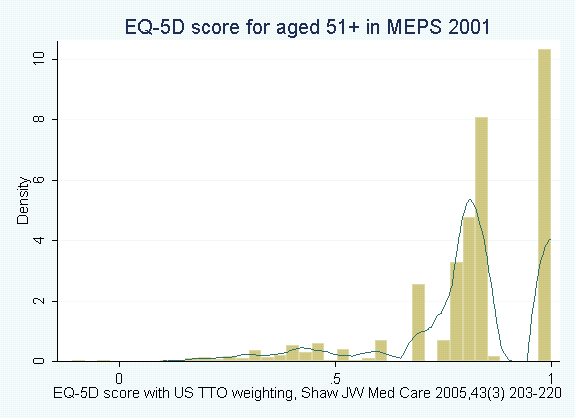
\includegraphics[scale=0.8]{./img/meps2001_age51p_eq5d_hist.png}
\caption{Distribution of EQ-5D index scores for ages 51+ in 2001 MEPS}
\label{fig:meps2001_age51p_eq5d_hist} 
\end{figure}

\subsubsection{MEPS-HRS Crosswalk development}
\label{sec:model_development_qalys_crosswalk}
The functional status measure in FEM is based on the HRS. It is a categorical 
variable including the following mutually exclusive categories: healthy, any IADL 
limitation (no ADL limitations), 1-2 ADL limitations, and 3 or more ADL limitations. 
Unfortunately the measures of IADL and ADL limitations in MEPS are quite different. 
HRS asks questions like ``Do you have any difficulty in $\ldots$'', while MEPS asks 
questions like ``Does $\ldots$help or supervision in $\ldots$.'' As Table 
\ref{tab:meps_hrs_adl_iadl_prevalence} shows, the prevalence of 
IADL limitations is relatively similar between the two surveys, while the 
prevalence of ADL limitations is much higher in HRS, relative to MEPS. This is 
reasonable since not all who have difficulty in ADLs receive help or supervision. 

In order to compute EQ-5D index scores using functional status in the FEM, we needed
a set of functional status measures that is comparable across MEPS and HRS (the host 
dataset for FEM).  We explored several options for deriving such a measure.  Ultimately,
we constructed two measures. One measure indicates physical function limitation 
while the other measure indicates IADL limitation. 

In MEPS, physical function 
limitation indicates that at least one of the following is true: 1) receiving help 
or supervision with bathing, dressing or walking around the house; 2) being limited 
in work/housework; 3) having difficulty walking, climbing stairs, grasping objects, 
reaching overhead, lifting, bending or stooping, or standing for long periods of time; 
or 4) having difficulty in hearing or vision. In HRS, physical function limitation indicates 
that at least one of the following is 
true: 1) having any difficulty in bathing/dressing/eating/walking across the room/getting 
out of bed; 2) limited in work/housework; or 3) limited in any other activities.

In MEPS, IADL limitation indicates receiving help or supervision using the telephone, 
paying bills, taking medications, preparing light meals, doing laundry, or going shopping.
In HRS, IADL limitation indicates having difficulty in any IADL such as using the phone, managing 
money, or taking medications. 

The prevalence of our two constructed measures among ages 51 and older in MEPS (2001) and HRS (1998) is 
shown in Table \ref{tab:meps_hrs_physlim_iadl_prevalence}. The prevalences are quite similar across the two surveys. 

Using MEPS 2001 data, we next use ordinary least squares to model the derived EQ-5D score as a function of six 
chronic conditions -- which are available both in HRS and MEPS, our two constructed measures of functional status, 
and an interaction term of the two measures of functional status. Three different models were considered. 
Estimation results are presented in Models I-III in Table \ref{tab:meps_eq5d_model_est}. We also show the estimation results of using only 
IADL/ADL limitation as covariates, and using only the six chronic conditions as covariates, as Models IV and V in 
Table \ref{tab:meps_eq5d_model_est}. Model II was used as the crosswalk described 
in Section \ref{sec:estimation_qalys} to calculate EQ-5D score for non-nursing 
home residents aged 51 and over in HRS 1998.




\subsection{Drug Expenditures}
\label{sec:model_development_rxexp}

\subsubsection{Drug Expenditures - MEPS}
\label{sec:model_development_rxexp_meps}
AHRQ produces a file of consolidated annual expenditures for each Medical Expenditure Panel Survey respondent in each calendar year.  
The total drug expenditure variable sums all amounts paid out-ot-pocket and by third party payers for each prescription
purchased in that year.  For comparison across years, we convert all amounts to 2010 dollars using the Medical CPI.

\subsubsection{Drug Expenditures - MCBS}
\label{sec:model_development_rxexp_mcbs}
The Medicare Current Beneficiary Survey produces a Prescribed Medicine Events file at the individual-event level, with cost
and utilization of prescribed medicines for the MCBS community population.  Collapsing this file to the individual provides an
estimate of prescription drug cost for each person.  For comparison across years, we convert all amounts to 2010 dollars using the Medical CPI.


There are two caveats to working with these data.  The first caveat regards how to handle the "ghost" respondents.  
"Ghosts" are individuals who enroll in Medicare, but were not
asked cost and use questions in the year of their enrollment.  For some outcomes, such as medical expenditures, the MCBS makes an 
effort to impute.  For others, such as drug utilization and expenditures, the MCBS does not.  We imputed annual drug expenditures 
for the ghosts, but for certain age ranges the drug expenditures were not reasonable.  This had the biggest effect on the 65 and 66 
year olds, for two reasons.  The first is that the 65 and 66 year olds are more likely to be ghosts, as 65 is the typical age of 
enrollment for Medicare.  The second is that the 65 and 66 year olds used for imputation (i.e., the non-"ghosts") are different.  To 
be fully present in MCBS at age 65 would require enrolling in Medicare before age 65, which happen through a different channel, such
as qualifying for Medicare due to receiving disability benefits from the federal government.  

The second caveat relates to the filling in zeroes for individuals with no utilization data, but who were enrolled.  We assumed that
individuals who were not ghosts and who did not appear on the Prescribed Medicine Events file had zero prescription expenditures.  
  

\subsubsection{Drug Expenditures - Estimation}
\label{sec:model_development_rxexp_estimation}
Due to the complexities of the age 65-66 population in the MCBS, we chose to estimate the drug expenditure models using the MEPS for 
individuals 51 to 66 and the MCBS for individuals 67 and older.  Individuals under age 65 receiving Medicare due to disability are 
estimated separately.  Since there are a number of individuals with zero expenditures, we estimate the models in two stages.  The 
first stage is a probit predicting any drug expenditures and the second is an ordinary least squares model predicting the amount, 
conditional on any.  Coefficient estimates and marginal effects are shown in the accompanying Excel workbook.




\section{Validation}
We perform cross-validation and external corroboration exercises.  Cross-validation is a test of the simulation�s internal validity that compares 
simulated outcomes to actual outcomes.  External corroboration compares model forecasts to others� forecasts.

\subsection{Cross-validation}
The cross-validation exercise randomly samples half of the PSID respondent IDs for use in estimating the transition models.  The respondents not used for estimation, 
but who were present in the PSID sample in 1999, are then simulated from 1999 through 2013.  Demographic, health, and economic outcomes are compared between the 
simulated (�FAM�) and actual (�PSID�) populations.  

%These results are presented in Table \ref{tab:crossval_unweighted} - Table \ref{tab:crossval_cntecon} for 2000, 2006, and 2012, 
%with a statistical test of the difference between the average values in the two populations.

Worth noting is how the composition of the population changes in this exercise.  In 1999, the sample represents those 25 and older.  Since we follow a fixed cohort, 
the age of the population will increase to 39 and older in 2013.  This has consequences for some measures in later years where the eligible population shrinks.

\subsubsection{Demographics}
Mortality and demographic measures are presented in Tables \ref{tab:crossval_unweighted} and \ref{tab:crossval_demog}.  Mortality incidence is comparable between
the simulated and observed populations.  Demographic characteristics do not differ between the two.

\subsubsection{Health Outcomes}
Binary health outcomes are presented in Table \ref{tab:crossval_binhlth}. FAM underestimates the prevalence of ADL and IADL limitations compared to the crossvalidation sample. 
Binary outcomes, like cancer, diabetes, heart diesease, and stroke do not differ.  FAM underpredicts hypertension and lung disease compared to the crossvalidation sample.

\subsubsection{Health Risk Factors}
Risk factors are presented in Table \ref{tab:crossval_risk}.  BMI is not statistically different between the two samples.  Current smoking is not statistically different,
 but more individuals in the crossvalidation sample report being former smokers.

\subsubsection{Economic Outcomes}
Binary economic outcomes are presented in Table \ref{tab:crossval_binecon}.  FAM underpredicts claiming of federal disability and overpredicts Social Security retirement 
claiming.  Supplemental Security claiming is not statistically different between FAM and the crossvalidation sample.  Working for pay is not statistically different.

%Continuout economic outcomes are presented in Table \ref{tab:crossval_cntecon}.

On the whole, the crossvalidation exercise is reassuring.  There are differences that will be explored and improved upon in the future.

%\subsection{External Validation}
NOTE: THIS SECTION NEEDS TO BE DEVELOPED

The external validation exercise compares FAM full population simulations beginning in 1999 to external sources.  

%\subsubsection{Benefits from Social Security Administration}

\subsubsection{Benefits from Medicare and Medicaid}

Compare benefits to Medicare and Medicaid.
\subsection{External Corroboration}
Finally, we compare FEM population forecasts to Census forecasts of the US population..  Here, we focus on the full HRS population (51 and older) and those 65 and 
older.  For this exercise, we begin the simulation in 2010 and simulate the full population through 2050.  Population projections are compared to the 2012 Census 
projections for years 2012 through 2050.  FEM population forecasts are always within two percent of Census forecasts.

\section{Baseline Forecasts}
In this section we present baseline forecasts of the Future Americans Model.  The figures show data from the PSID for the 25+ population from 1999 through 2009 and 
forecasts from the FAM for the 25+ population beginning in 2009.

\subsection{Disease Prevalence}
Figure \ref{fig:chronic_diseases_male} depicts the six chronic conditions we project for men.  And Figure \ref{fig:chronic_diseases_female} depicts the historic 
and forecasted values for women.

\begin{figure}[ht!]
\centering

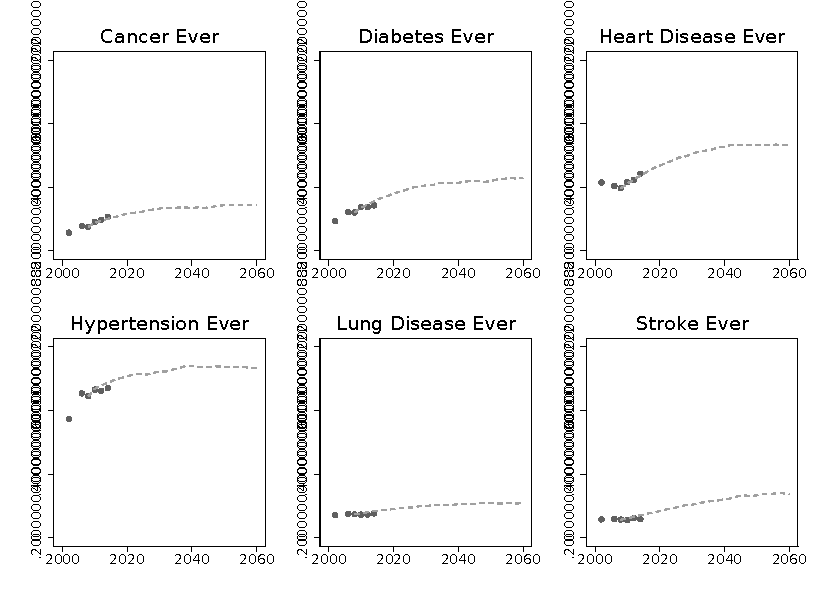
\includegraphics[scale=1.0]{./img/chronic_diseases_male}
\caption{Historic and Forecasted Chronic Disease Prevalence for Men 25+}
\label{fig:chronic_diseases_male} 

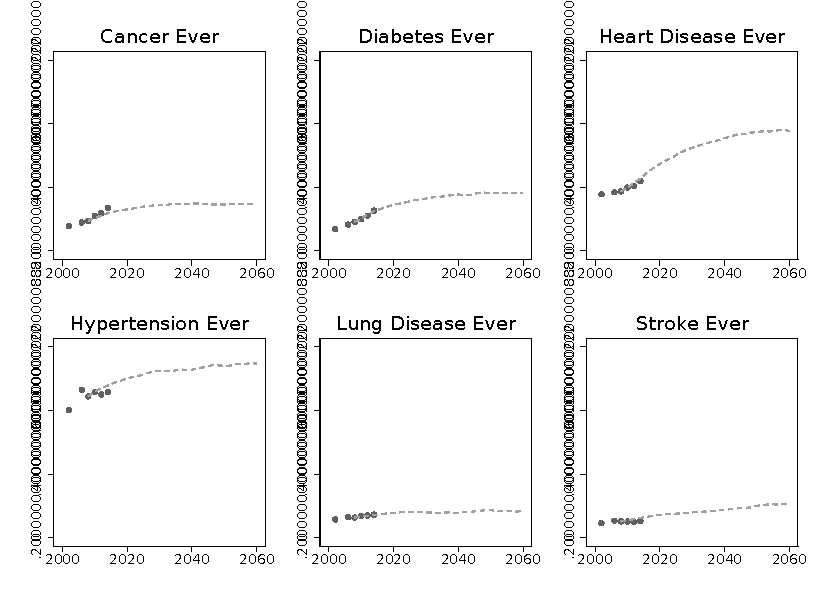
\includegraphics[scale=1.0]{./img/chronic_diseases_female}
\caption{Historic and Forecasted Chronic Disease Prevalence for Women 25+}
\label{fig:chronic_diseases_female} 
\end{figure}

Figure \ref{fig:adl_iadl_male} shows historic and forecasted levels for any ADL difficulties, three or more ADL difficulties, any IADL difficulties, and
two or more IADL difficulties for men 25 and older. Figure \ref{fig:adl_iadl_female} shows historic and forecasted levels for any ADL difficulties, three or 
more ADL difficulties, any IADL difficulties, and two or more IADL difficulties for women 25 and older.

\begin{figure}[ht!]
\centering

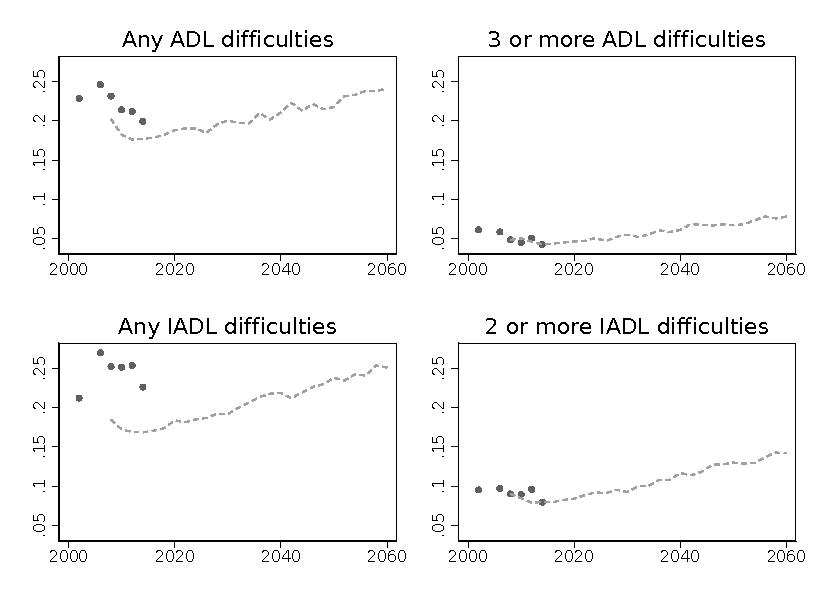
\includegraphics[scale=1.0]{./img/adl_iadl_male}
\caption{Historic and Forecasted ADL and IADL Prevalence for Men 25+}
\label{fig:adl_iadl_male} 

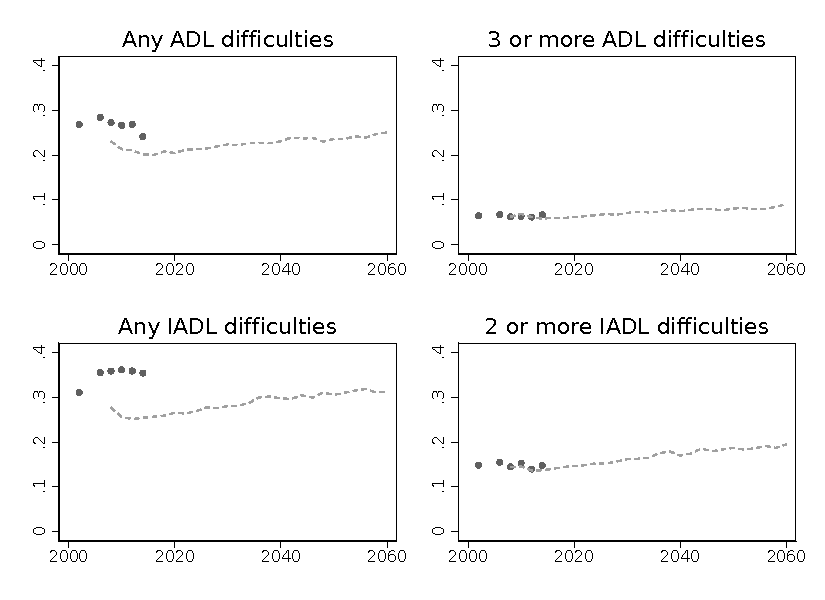
\includegraphics[scale=1.0]{./img/adl_iadl_female}
\caption{Historic and Forecasted ADL and IADL Prevalence for Women 25+}
\label{fig:adl_iadl_female} 
\end{figure}

\section{Acknowledgments}

The Future Elderly Model and Future Americans Model has been developed by a large team over the last decade.  Jay Bhattacharya, Eileen Crimmins, Christine Eibner, \'Etienne Gaudette, Geoff Joyce, Darius Lakdawalla,
Pierre-Carl Michaud, and Julie Zissimopoulos have all provided expert guidance.  Adam Gailey, Baoping Shang, and Igor Vaynman provided programming and analytic 
support during the first years of FEM development at RAND.  Jeff Sullivan then led the technical development for several years.  More recently, the University of 
Southern California research programming team has supported model development, including FAM development.  These programmers include Patricia St. Clair, Laura Gascue, Henu Zhao, and Yuhui Zheng. 
Barbara Blaylock, Malgorzata Switek, and Wendy Cheng have greatly aided model development while working as research assistants at USC.


\section{Tables}

% FAM initial conditions are:
%Economic: 	Work Status, 	Earnings, 				Wealth
%Health: 		BMI Category, Smoking Category, Hypertension 
%Other: 		Education, 		Partnered, 				Partner Type, Health Insurance

\begin{table}[h]\centering
\begin{tabular}{l l l}
\textbf{Economic Outcomes} & \textbf{Health Outcomes} & \textbf{Other Outcomes}\\
Work Status & BMI Category & Education\\
Earnings & Smoking Category & Partnered\\
Wealth & Hypertension & Partner Type\\
& & Health Insurance
\end{tabular}~\\~\\
\caption{Estimated outcomes in replenishing cohorts module}
\label{tab:initial_conditions_model}
\end{table}

% FAM transition models are:
%Economic: Social Security Claiming, Disability Claiming, Supplemental Security Income Claiming, Non-Zero Capital Income, Capital Income, Non-zero Government Transfers, Government Transfers, Non-zero Wealth, Wealth, Laborforce Status, Full- or Part-time, Any Earnings if Unemployed, Any Earnings if Not in Labor Force, Earnings if Full-time, Earnings if Part-time, Earnings if Unemployed, Earnings if Not in Labor Force
%Health: Mortality, Heart Disease, Stroke, Cancer, Hypertension, Diabetes, Lung Disease, Start Smoking, Stop Smoking, ADL Status, IADL Status, Births/Paternity, Self-reported Health, BMI, Partner Death
%Marital Status (by sex): Exit Single, Exit Cohabitation, Exit Married, Single to Married, Cohabitation to Married, Married to Cohabitation
%Other: Insurance Type

\begin{sidewaystable}
\centering
\begin{tabular}{l l l l}
\textbf{Economic Outcomes} & \textbf{Health Outcomes} &  \textbf{Marital Status} & \textbf{Other Outcomes}\\
Social Security Claiming & Mortality & Exit Single & Insurance Type\\
Disability Claiming & Heart Disease & Exit Cohabitation &\\
Non-Zero Capital Income & Cancer & Exit Married & \\
Capital Income (if non-zero) & Hypertension & Single to Married &\\
Non-zero Government Transfers & Diabetes & Cohabitation to Married & \\
Government Transfers (if non-zero) & Lung Disease & Married to Cohabitation & \\
Non-zero Wealth & Start Smoking & & \\
Wealth (if non-zero) & Stop Smoking & &\\
Labor Force Status (out, unemployed, working) & ADL Status & &\\
Employed Full- or Part-time (if working) & IADL Status & &\\
Any Earnings (if Unemployed) & Births/Paternity & &\\
Any Earnings (if Not in Labor Force) & Self-reported Health & &\\
Earnings (if Full-time) & BMI & &\\
Earnings (if Part-time) & Partner Death & &\\
Earnings (if Unemployed and any) & & &\\
Earnings (if Not in Labor Force and any) & & &\\
\end{tabular}
\caption{Estimated outcomes in transitions module}
\label{tab:transition_model}
\end{sidewaystable}


\begin{sidewaystable}
\centering
\begin{tabular}[h]{l rrrrrrrr}
\input{../tables/FAM/svy_disease_prevalence.tex}
\end{tabular}
\caption{Health condition prevalences in survey data}
\label{tab:svy_disease_prevalence}
\end{sidewaystable}



\begin{sidewaystable}
\centering
\scalebox{0.75}{
\begin{tabular}{l p{2.5in}p{2.5in}p{2.5in}p{2.5in}}
& \multicolumn{4}{c}{Survey}\\
Disease & \multicolumn{1}{c}{PSID/HRS} & \multicolumn{1}{c}{NHIS} & \multicolumn{1}{c}{MEPS} & \multicolumn{1}{c}{MCBS} \\
\hline
Cancer &
Has a doctor ever told you that you have cancer or a malignant tumor, excluding minor skin cancers?&
Have you ever been told be a doctor or other health professional that you had � cancer or a malignanacy of any kind? (WHEN RECODED, SKIN CANCERS WERE EXCLUDED)&
List all the conditions that have bothered (the person) from (START time) to (END time) CCS codes for the conditions list are 11-21, 24-45&
Has a doctor ever told you that you had any (other) kind of cancer malignancy, or tumor other than skin cancer?\\
\hline
Heart Diseases &
Has a doctor ever told you that you had a heart attack, coronary heart disease, angina, congestive heart failure, or other heart problems?&
Four separate questions were asked about whether ever told by a docotor or oither health professional that had: CHD, Angina, MI, other heart problems.&
Have you ever been told by a doctor or health professional that you have � CHD; Angina; MI; other heart problems&
Six separate questions were asked about whether ever told by a doctor that had: Angina or MI; CHD; other heart problems (included four questions)\\
\hline
Stroke &
Has a doctor ever told you that you had a stroke?&
Have you EVER been told by a doctor or other health professional that you had a stroke?&
If Female, add: [Other than during pregnancy,] Have you ever been told by a doctor or health professional that you have a stroke or TIA (transient ischemic attack)&
[Since (PREV$<$ SUPP. RD. INT. DATE),] has a doctor (ever) told (you/SP) that (you/he/she) had a stroke, a brain hemorrhage, or a cerebrovascular accident?\\
\hline
Diabetes&
Has a doctor ever told you that you have diabetes or high blood sugar?&
If Female, add: [Other than during pregnancy,] Have you ever been told by a doctor or health professional that you have diabetes or sugar diabetes?&
If Female, add: [Other than during pregnancy,] Have you hever been told by a doctor or health professional that you have diabetes or sugar diabetes?&
Has a doctor (ever) told (you/SP) that (you/he/she) had diabetes, high blood sugar, or sugar in (your/his/her) urine? [DO NOT INCLUDE BOERDERLINE PREGNANCY, OR PRE-DIABETEIC DIABETES.]\\
\hline
Hypertension&
Has a doctor ver told you that you have high blood pressure or hypertension?&
Have you EVER been told by a doctor or other health professional that you had Hypertension, also called high blood pressure?&
Have you EVER been told by a doctor or other health professional that you had Hypertension, also called high blood pressure?&
Has a doctor (ever) told (you/SP) that (you/he/she) (still) (had) (have/has) hypertension, sometimes called high blood pressure?\\
\hline
Lung Disease&
Has a doctor ever told you that you have chronic lung disease such a schronic bronchitis or emphysema? [IWER: DO NOT INCLUDE ASTHMA]&
Question 1: During the PAST 12 MONTHS, have you ever been told by a doctor or other health professional that you had chronic bronchitis? Question 2: Have you EVER been told by a docotor or other health professional that you had � emphysema?&
List all the conditions that have bothered (the person) from (START time) to (END time) CCS codes for the conditions list are 127, 129-312&
Has a doctor (ever) told (you/SP) that (you/he/she) had emphysema, asthma, or COPD? [COPD=CHRONIC OBSTRUCTIVE PULMONARY DISEASE.]\\
\hline
Overweight & \multicolumn{4}{c}{\multirow{2}{*}{Self-reported body weight and height}}\\
\hhline{-~~~~}
Obese & \multicolumn{4}{c}{} \\
\hline
\end{tabular}
}
\caption{Survey questions used to determine health conditions}
\label{tab:svy_disease_questions}
\end{sidewaystable}


\begin{sidewaystable}
% \todo Dynamically fill in numeric results using Sweave
\centering
\scalebox{0.9}{
\begin{tabular}{lllccr}
 &  &  & Type & At risk & Mean/fraction\\
\hline
\input{../tables/FAM/transitioned_outcomes_disease.tex}
\hline
\input{../tables/FAM/transitioned_outcomes_smoking.tex}
\hhline{~-----}
\input{../tables/FAM/transitioned_outcomes_logbmi.tex}
\hhline{~-----}
\input{../tables/FAM/transitioned_outcomes_adlstat.tex}
\hhline{~-----}
\input{../tables/FAM/transitioned_outcomes_iadlstat.tex}
\hline
\input{../tables/FAM/transitioned_outcomes_work.tex}
\hhline{~-----}
\input{../tables/FAM/transitioned_outcomes_lfpben.tex}
\hline
\input{../tables/FAM/transitioned_outcomes_mstat.tex}
\hhline{~-----}
\input{../tables/FAM/transitioned_outcomes_birth.tex}
\hline
\input{../tables/FAM/transitioned_outcomes_financial.tex}
\hline
\end{tabular}
}
\caption[Outcomes in the transition model]{Outcomes in the transition model. Estimation sample is PSID 1999-2013 waves.}
\label{tab:transitioned_outcomes}
\end{sidewaystable}


\begin{sidewaystable}
% \todo Write a script that dynamically generates this table from the .est files
\centering
\scalebox{0.53}{
\begin{tabular}{l*{20}{c}}
Value at time $T-1$ & \multicolumn{20}{c}{Outcome at time $T$}  \\
\hline
 & Heart  &  & & Lung  & & &  &  & Smoking  &  &  & &  &  & & Nursing & & &  Nonzero & \\
 & disease & hypertension & stroke & disease & diabetes & cancer & disability & mortality & status & BMI & Any HI & DI Claim & SS Claim & DB Claim & SSI Claim & Home & Work & Earnings & Wealth & Wealth\\
Heart disease &  &  & \checkmark &  &  &  & \checkmark & \checkmark & \checkmark & \checkmark & \checkmark & \checkmark & \checkmark & \checkmark & \checkmark & \checkmark & \checkmark & \checkmark & \checkmark & \checkmark\\
Blood pressure & \checkmark &  & \checkmark &  &  &  & \checkmark & \checkmark & \checkmark & \checkmark & \checkmark & \checkmark & \checkmark & \checkmark & \checkmark & \checkmark & \checkmark & \checkmark & \checkmark & \checkmark\\
Stroke &  &  &  &  &  &  & \checkmark & \checkmark & \checkmark & \checkmark & \checkmark & \checkmark & \checkmark & \checkmark & \checkmark & \checkmark & \checkmark & \checkmark & \checkmark & \checkmark\\
Lung disease &  &  &  &  &  &  & \checkmark & \checkmark & \checkmark & \checkmark & \checkmark & \checkmark & \checkmark & \checkmark & \checkmark & \checkmark & \checkmark & \checkmark & \checkmark & \checkmark\\
Diabetes & \checkmark & \checkmark & \checkmark &  &  &  & \checkmark & \checkmark & \checkmark & \checkmark & \checkmark & \checkmark & \checkmark & \checkmark & \checkmark & \checkmark & \checkmark & \checkmark & \checkmark & \checkmark\\
Cancer &  &  & \checkmark &  &  &  & \checkmark & \checkmark & \checkmark & \checkmark & \checkmark & \checkmark & \checkmark & \checkmark & \checkmark & \checkmark & \checkmark & \checkmark & \checkmark & \checkmark\\
Disability &  &  &  &  &  &  & \checkmark & \checkmark & \checkmark & \checkmark & \checkmark & \checkmark & \checkmark & \checkmark & \checkmark & \checkmark & \checkmark & \checkmark & \checkmark & \checkmark\\
Claimed DI &  &  &  &  &  &  &  &  &  &  & \checkmark & \checkmark & \checkmark & \checkmark & \checkmark &  & \checkmark & \checkmark & \checkmark & \checkmark\\
Claimed SS &  &  &  &  &  &  &  &  &  &  & \checkmark &  &  & \checkmark & \checkmark &  & \checkmark & \checkmark & \checkmark & \checkmark\\
Claimed DB &  &  &  &  &  &  &  &  &  &  &  &  & \checkmark &  & \checkmark &  & \checkmark & \checkmark & \checkmark & \checkmark\\
Claimed SSI &  &  &  &  &  &  &  &  &  &  &  &  &  &  & \checkmark &  &  &  &  & \\
Work &  &  &  &  &  &  &  &  &  &  & \checkmark & \checkmark & \checkmark &  & \checkmark &  & \checkmark & \checkmark & \checkmark & \checkmark\\
Earnings &  &  &  &  &  &  &  &  &  &  & \checkmark & \checkmark & \checkmark & \checkmark & \checkmark &  & \checkmark & \checkmark & \checkmark & \checkmark\\
Nonzero wealth &  &  &  &  &  &  &  &  &  &  & \checkmark & \checkmark & \checkmark & \checkmark & \checkmark & \checkmark & \checkmark & \checkmark & \checkmark & \checkmark\\
Wealth &  &  &  &  &  &  &  &  &  &  & \checkmark & \checkmark & \checkmark & \checkmark & \checkmark & \checkmark & \checkmark & \checkmark & \checkmark & \checkmark\\
Nursing home stay &  &  &  &  &  &  &  &  &  &  &  &  &  &  & \checkmark & \checkmark &  &  & \checkmark & \checkmark
\end{tabular}
}
\caption[Restrictions on transition model]{Restrictions on transition model. \checkmark indicates that an outcome at time $T-1$ is allowed in the transition model for an outcome at time $T$.}
\label{tab:transition_restrictions}
\end{sidewaystable}

\begin{table}
\centering
\scalebox{1}{
\input{../tables/FAM/controlvar_descs.tex}
}
\caption[Descriptive statistics for stock population]{Desciptive statistics for variables in 2009 PSID ages 25+ sample used as simulation stock population}
\label{tab:controlvar_descs}
\end{table}


%\begin{table}
%% \todo Dynamically fill in numeric results using Sweave and reduce the number of sig. digits after decimal
%\centering
%\scalebox{0.9}{
%\begin{tabular}{ccccrr}
% &  &  & Selection & 1992 & 2004 \\
%\hline
%\input{../tables/FAM/desc_init_conditions_binary.tex}
%\hline
%\input{../tables/FAM/desc_init_conditions_bmistat.tex}
%\hhline{~-----}
%\input{../tables/FAM/desc_init_conditions_smoking.tex}
%\hhline{~-----}
%\input{../tables/FAM/desc_init_conditions_funcstat.tex}
%\hline
%\input{../tables/FAM/desc_init_conditions_continuous.tex}
%\hline
%\input{../tables/FAM/desc_init_conditions_censcont.tex}
%\hline
%\input{../tables/FAM/desc_init_conditions_censdiscrete.tex}
%\hline
%\input{../tables/FAM/desc_init_conditions_earlyagedb.tex}
%\hhline{~-----}
%\input{../tables/FAM/desc_init_conditions_normalagedb.tex}
%\hline
%\input{../tables/FAM/desc_init_conditions_covars.tex}
%\hline
%\end{tabular}
%}
%\caption{Initial conditions used for estimation (1992) and simulation (2004)}
%\label{tab:desc_init_conditions}
%\end{table}


\begin{sidewaystable}
\centering
\scalebox{1}{
\input{../tables/FAM/latent_model_mean_est.tex}
}
\caption[Parameter estimates for latent model: conditional means and thresholds]{Parameter estimates for latent model: conditional means and thresholds. Sample is respondents age 25-30 in 2005-2011 PSID waves}
\label{tab:latent_model_mean_est}
\end{sidewaystable}


\begin{sidewaystable}
\centering
\scalebox{1}{
\input{../tables/FAM/latent_model_vcmat_est.tex}
}
\caption[Parameter estimates for latent model: parameterized covariance matrix]{Parameter estimates for latent model: parameterized covariance matrix. Sample is respondents age 25-30 in 2005-2011 PSID waves}
\label{tab:latent_model_vcmat_est}
\end{sidewaystable}



\begin{sidewaystable}
\centering
\input{../tables/FAM/new_cohort_trends_health.tex}
\caption{Health and risk factor trends for replenishing cohorts, prevalences relative to 2009}
\label{tab:new_cohort_trends_health}
\end{sidewaystable}

\begin{sidewaystable}
\centering
\input{../tables/FAM/new_cohort_trends_educ.tex}
\caption{Education trends for replenishing cohorts, prevalences relative to 2009}
\label{tab:new_cohort_trends_educ}
\end{sidewaystable}

\begin{sidewaystable}
\centering
\input{../tables/FAM/new_cohort_trends_social.tex}
\caption{Social trends for replenishing cohorts, prevalences relative to 2009}
\label{tab:new_cohort_trends_social}
\end{sidewaystable}



%\begin{table}
%\centering
%\input{../tables/FAM/NHEA_adjustment.tex}
%\caption{Per capita medical spending by payment source, age group, and year}
%\label{tab:NHEA_adjustment}
%\end{table}



%\begin{table}
%\centering
%\scalebox{0.8}{
%\input{../tables/FAM/time_series_by_year.tex}
%}
%\caption{Assumptions for each calendar year}
%\label{tab:time_series_by_year}
%\end{table}

%\begin{table}
%\centering
%\scalebox{0.8}{
%\input{../tables/FAM/time_series_by_yob.tex}
%}
%\caption[Assumptions for each birth year]{Assumptions for each birth year. In years after 1960, all values are held constant at their 1960 levels.}
%\label{tab:time_series_by_yob}
%\end{table}


\begin{table}
\centering
\input{../tables/FAM/crossval_unweighted.tex}
\caption{Crossvalidation of 1999 cohort: Mortality in 2001, 2007, and 2013}
\label{tab:crossval_unweighted}
\end{table}


\begin{table}
% \todo clean up the significant digits in this table
% \todo create a variable sort order (file that maps variable names to integers) that can be merged on and then labels can be sorted in this table
\centering
\input{../tables/FAM/crossval_demog.tex}
\caption{Crossvalidation of 1999 cohort: Demographic outcomes in 2001, 2007, and 2013}
\label{tab:crossval_demog}
\end{table}


\begin{table}
% \todo clean up the significant digits in this table
% \todo create a variable sort order (file that maps variable names to integers) that can be merged on and then labels can be sorted in this table
\centering
\input{../tables/FAM/crossval_binhlth.tex}
\caption{Crossvalidation of 1999 cohort: Binary health outcomes in 2001, 2007, and 2013}
\label{tab:crossval_binhlth}
\end{table}

\clearpage

\begin{table}
% \todo clean up the significant digits in this table
% \todo create a variable sort order (file that maps variable names to integers) that can be merged on and then labels can be sorted in this table
\centering
\input{../tables/FAM/crossval_risk.tex}
\caption{Crossvalidation of 1999 cohort: Risk factor outcomes in 2001, 2007, and 2013}
\label{tab:crossval_risk}
\end{table}

\begin{table}
% \todo clean up the significant digits in this table
% \todo create a variable sort order (file that maps variable names to integers) that can be merged on and then labels can be sorted in this table
\centering
\input{../tables/FAM/crossval_binecon.tex}
\caption{Crossvalidation of 1999 cohort: Binary economic outcomes in 2001, 2007, and 2013}
\label{tab:crossval_binecon}
\end{table}


%\begin{table}
%% \todo clean up the significant digits in this table
%% \todo create a variable sort order (file that maps variable names to integers) that can be merged on and then labels can be sorted in this table
%\centering
%\input{../tables/FAM/crossval_cntecon.tex}
%\caption{Crossvalidation of 1999 cohort: Simulated vs reported continuous economic outcomes in 2001, 2007, and 2013}
%\label{tab:crossval_cntecon}
%\end{table}




\begin{sidewaystable}
\centering
\input{../tables/FAM/external_pop.tex}
\caption{Population forecasts: Census compared to FAM}
\label{tab:external_pop}
\end{sidewaystable}


 
\appendix
%\input{./myappendix.tex}
 
 
% Bibliography:
\clearpage
\section*{}
\addcontentsline{toc}{section}{References}
\bibliographystyle{apalike}
\bibliography{../../../fem_bibliography.bib}
%\input{./mybibliography.tex}
 
\end{document}
